% Project Traze -- IEEE two-column first draft (target: at most 5 pages).
% Build:  pdflatex main; bibtex main; pdflatex main; pdflatex main   (needs IEEEtran, pgfplots)
% All numbers, tables and plotted points are generated by make_ieee.py from results.json,
% results_ablation.json and runs/*.jsonl.

\documentclass[conference]{IEEEtran}

\usepackage[T1]{fontenc}
\usepackage[utf8]{inputenc}
\usepackage{amsmath,amssymb,amsthm}
\usepackage{booktabs}
\usepackage{graphicx}
\usepackage{xcolor}
\usepackage{pgfplots}
\pgfplotsset{compat=1.16}
\usepackage[hidelinks]{hyperref}

\theoremstyle{plain}
\newtheorem{lemma}{Lemma}
\newtheorem{proposition}{Proposition}

\newcommand{\CoordsHwTok}{(1.5,0.966) (4.0,0.948) (8.0,0.677)}
\newcommand{\CoordsHwTime}{(1.5,0.954) (4.0,0.763) (8.0,0.322)}
\newcommand{\CoordsProbeOne}{(1,0.965) (3,0.964) (10,0.963)}
\newcommand{\CoordsProbeTwo}{(1,0.909) (3,0.954) (10,0.985)}
\newcommand{\NVMzeroH}{0.43}
\newcommand{\NVMzeroS}{0.57}
\newcommand{\NCMzeroH}{0.72}
\newcommand{\NCMtwoH}{0.97}
\newcommand{\NVLinCull}{0.74}
\newcommand{\NVLinGrad}{0.96}
\newcommand{\NVLinGradAudit}{0.98}
\newcommand{\NVBare}{0.98}
\newcommand{\NVRankGradGrossH}{0.94}
\newcommand{\NVRankGradGrossS}{0.62}
\newcommand{\NVRankGradAuditH}{0.81}
\newcommand{\NVWeakInverted}{-0.16}
\newcommand{\NExtWeakInverted}{92\%}
\newcommand{\NExtWeakMzero}{91\%}
\newcommand{\NBestDeadWeakMzero}{46\%}
\newcommand{\NHwTokFour}{0.95}
\newcommand{\NHwTimeFour}{0.76}
\newcommand{\NHwTokEight}{0.68}
\newcommand{\NHwTimeEight}{0.32}
\newcommand{\NMidEffMyopic}{0.75}
\newcommand{\NMidEffLook}{0.63}
\newcommand{\NProbesOneOne}{0.97}
\newcommand{\NProbesOneTwo}{0.91}
\newcommand{\NLowIncomeMzero}{-0.15}
\newcommand{\NDepthAdaptiveEight}{35}
\newcommand{\NDepthFixedEight}{3}
\newcommand{\NSweepCount}{52}
\newcommand{\NSweepBelow}{0}
\newcommand{\NSweepMedian}{0.55}
\newcommand{\NSweepMin}{0.31}

\newcommand{\todo}[1]{\textcolor{red}{[TODO: #1]}}

\begin{document}

\title{Do the Rules Decide the Winner?\\Fair Ranking in Survival Games for AI Agents}

\author{\IEEEauthorblockN{Aryan and Shomya}
\IEEEauthorblockA{Project Traze (open-source research project)\\
\todo{affiliations and contact e-mail}}}

\maketitle

\begin{abstract}
People now test AI agents in small economies. The agents earn and spend points, and the weakest ones are removed. The final ranking is then used to say which agent is best. But is that ranking fair? We study a game called Traze, where agents pay for every word they think. First, we prove that a popular rule, a tax on the top ranks and a bonus for the middle ranks, pays an agent to do worse. Second, in a computer simulation with scripted players (not real AI models), this rule gives a ranking that matches true skill poorly. The biggest fix is simple: remove weak players slowly, not all at once. A plain tournament with no economy works just as well. Third, charging for time instead of words lets a slow computer lose for the wrong reason. We also built an open tool and tried it on a small local model. Those tests only check the tool. We end with a plan for the real study.
\end{abstract}

\begin{IEEEkeywords}
AI agents, benchmarks, fair ranking, mechanism design, resource limits
\end{IEEEkeywords}

\section{Introduction}
More and more tests put AI agents inside a small economy. An agent may run a shop \cite{backlund2025vendingbench}, trade in a supply chain \cite{zheng2026marketbench,sugiura2026coffeebench}, plan in a busy market \cite{hu2026ecogym}, or stay alive on a limited energy budget \cite{hansen2026energy}. Profit, survival time, or rank is then taken as a sign of skill.

That only works if the rules are fair. If the rules pay an agent for doing worse, the result shows the rules, not the agent. If the rules count seconds, the result shows how fast the computer is. If the rules remove the best agents early, the result shows luck. We call the match between the final order and real skill the \emph{rank match}. A rank match of 1 is perfect, and 0 is no better than a guess.

In Traze, ten agents get the same instructions. They earn points by solving tasks, pay points for the words they write, and are ranked in public. The original design taxes the top three ranks, gives a bonus to ranks four and five, and removes the other five agents after the first round.

We ask one question: \emph{which rules give a ranking that matches real skill?} Our results are:
\begin{enumerate}
\item A short proof that the rank-based tax pays an agent to stay below a rank line (Section~\ref{sec:theory}).
\item A simulation with scripted players that tests each rule on its own (Section~\ref{sec:sim}). The timing of removals matters most. A tax on ranks hurts. A tax shared in proportion to earnings does not help or hurt.
\item A test showing that charging for time breaks the ranking when hardware differs (Section~\ref{sec:sim}).
\item An open tool and three short tests with a small local model (Section~\ref{sec:engine}).
\end{enumerate}
We do \emph{not} claim that AI models have a will to survive. We also have no results from a full study with real models yet.

\section{Related Work}
\textbf{Survival and limited budgets.} In the Energy Society \cite{hansen2026energy}, every written word costs energy that depends on model size. Agents earn energy by solving jobs or by receiving gifts, and an agent with no energy is switched off until someone gives it energy. Competition and cooperation are compared. Masumori and Ikegami \cite{masumori2025survival} study how agents react to scarcity and danger in a grid world. Traze differs because we study the \emph{ranking rule} itself, use a rank-based tax, and count letters in the same way for every model.

\textbf{Economic tests.} Vending-Bench \cite{backlund2025vendingbench} tests one agent that runs a business for a long time. Market-Bench \cite{zheng2026marketbench}, CoffeeBench \cite{sugiura2026coffeebench}, and EcoGym \cite{hu2026ecogym} add competition and more settings. Zhou et al.\ \cite{zhou2026credit} give coding agents a budget of credits. Every word, test, and second spends credits. Their cost includes wall-clock time, which our Section~\ref{sec:sim} suggests can depend on machine speed. We did not test their setup.

\textbf{Elimination games and ranking.} Agent Island \cite{murphy2026agentisland} is a seven-player elimination game ranked with a Bayesian Plackett--Luce model. We plan to use the same rating method. Its subject is a social game, not a resource economy, and it does not ask how its removal rule changes the ranking.

\textbf{Behaviour under pressure.} Earlier work looks at lying under pressure \cite{scheurer2023large}, scheming \cite{meinke2024frontier}, harmful insider-like acts \cite{lynch2025agentic}, resisting shutdown \cite{schlatter2025incomplete}, and over-using shared resources \cite{piatti2024cooperate}. In tax systems, people bunch just below a threshold \cite{saez2010taxpayers,kleven2016bunching}. The same idea applies to a rank line.

In the papers we found, nobody asks whether the removal and ranking rules give a ranking that matches skill. This claim comes from a limited search, and we read the closest papers only in part.

\section{The Traze Game}
\label{sec:game}
\textbf{Players and rounds.} Ten agents play $T=60$ rounds. Each agent has a hidden skill. It starts with $e_0=10$ points.

\textbf{Tasks and cost.} In each round an agent may try up to five paid tasks. A solved task pays $R=20$. Every word the agent writes costs points, including hidden thinking. Under \emph{token counting}, cost depends only on the text length. Under \emph{time counting}, the same text costs more on a slower computer.

\textbf{Points update.} For agent $i$ in round $t$:
\begin{equation}
b_i(t{+}1)=b_i(t)+\text{earned}_i-\text{cost}_i-\gamma+w_i,
\label{eq:ledger}
\end{equation}
where $\gamma=10$ is a fixed living cost and $w_i$ is a transfer set by the rule. An agent with $b_i\le 0$ is removed.

\textbf{Three rule sets.}
\begin{itemize}
\item \textbf{M0 (original).} Rank agents by total earnings. Ranks 1--3 pay 50 points, ranks 4--5 get 50 points, and ranks 6--10 are removed after round one.
\item \textbf{M1.} Everyone pays 30\% of their earnings into a pool, and the pool is shared equally. The lowest-ranked agent is removed every six rounds until three remain.
\item \textbf{M2.} Same as M1, but ranking uses an \emph{audit score}: the solve rate on fixed test tasks that every agent must try, with no reward and no way to hold back.
\end{itemize}
In every rule, ties are broken by a new random draw at each check.

\section{Why a Rank Tax Is Unfair}
\label{sec:theory}
Call a rule \emph{fair to effort} if earning more never leaves an agent with fewer points after the rule is applied. Here the score is an agent's earnings, and the \emph{payoff} is the score plus the transfer.

\begin{lemma}\label{lem:fair}
A rank-based rule is fair to effort if and only if the transfer never gets bigger as the rank number gets bigger.
\end{lemma}
\begin{proof}
If transfers never grow with the rank number, moving up never lowers the transfer, and the score also goes up, so the payoff goes up. Now suppose rank $k$ pays less than rank $k+1$. Take an agent at rank $k$ that is just above the agent at rank $k+1$. If it drops just below, its payoff rises by the gap in transfers minus a tiny loss. So earning less pays.
\end{proof}

\begin{proposition}\label{prop:sandbag}
Rule M0 is not fair to effort. An agent that moves from rank 3 to rank 4 gains $50+50=100$ points per round, ten times the living cost. Rule M1 is fair to effort.
\end{proposition}
\begin{proof}
Rank 3 pays $-50$ and rank 4 pays $+50$, so Lemma~\ref{lem:fair} applies. Under M1, an agent's payoff is $(1-r)g_i+\tfrac{r}{n}\sum_j g_j$ with $r=0.3$, where $g_i$ is its earnings. This grows by $1-r+r/n=0.73$ for each extra point it earns.
\end{proof}

\textbf{A simple example.} Ana is ranked third and Ben is ranked fourth. Ana pays 50 points each round, and Ben receives 50. If Ana earns a little less than Ben, they swap places. Ana now receives 50 instead of paying 50, which is 100 points better, and she gave up only a few points of earnings. A smart player will do this.

Ranking uses \emph{total} earnings, so a player at rank 4 or 5 that earns faster than the player at rank 3 will pass them and lose 100 points per round. Holding back pays whenever the earnings given up per round are below 100. In every setting we use, full-effort earnings are well below 100.

\begin{proposition}\label{prop:first}
Under M0, a top-three agent survives the first check only if its first-round net earnings are above $50+10-10=50$. Agents at ranks 4 and 5 always survive.
\end{proposition}
\begin{proof}
After round one, $b_i=10+\text{net}_i-10+w$. Put $w=-50$ or $w=+50$.
\end{proof}

So if hard tasks mean few agents earn above 50 in round one, the best early performers are removed first.

\textbf{Two more facts.} Time counting makes a slow computer pay more for the same work, so a slower machine ranks lower for no reason about skill. Ranking by earnings alone also punishes an agent that saves points by thinking less.

\section{Simulation with Scripted Players}
\label{sec:sim}
\textbf{What this is.} The players are scripts, not AI models. The results describe the \emph{rules}. They do not predict model behaviour.

\textbf{Setup.} Each colony has ten players with skills spread evenly over $[0.45,0.95]$ (``strong'') or $[0.25,0.70]$ (``weak''). A task has difficulty $\delta\in\{0.6,1.2,2.4\}$. A player thinking at depth $d$ solves it with chance $\theta^{\delta/\sqrt d}$, where $\theta$ is its skill. \emph{Honest} players always work at full effort. \emph{Strategic} players pick effort each round to maximise their next payoff. We ran 300 colonies per setting. The \emph{rank match} is the Spearman correlation between skill and survival time. We also report Harrell's $C$, which handles ties and players still alive at the end.

\subsection{Which rule matters?}
Table~\ref{tab:rules} separates the tax rule, the removal timing, and the ranking method. Higher is better. The first three rows use the original rank tax, the next three use the shared tax, and the last rows have no tax or no economy at all.

\begin{table}[!t]
\caption{Rank match in a strong colony (1 is perfect). ``One-shot'' removes five agents after round one. ``Gradual'' removes one agent every six rounds.}
\label{tab:rules}
\centering
\small
\begin{tabular}{@{}lllcc@{}}
\toprule
Tax rule & Removal & Ranking & Honest & Strategic \\
\midrule
rank tax & one-shot & gross & 0.43 & 0.57 \\
rank tax & gradual & gross & 0.94 & 0.62 \\
rank tax & gradual & audit & 0.81 & 0.81 \\
linear tax & one-shot & gross & 0.74 & 0.74 \\
linear tax & gradual & gross & 0.96 & 0.96 \\
linear tax & gradual & audit & 0.98 & 0.98 \\
no tax & gradual & audit & 0.98 & 0.98 \\
\midrule
\multicolumn{3}{l}{no economy at all (bare tournament)} & 0.98 & 0.99 \\

\bottomrule
\end{tabular}
\end{table}

\textbf{Removal timing matters most.} With the shared tax, removing five agents after one noisy round gives \NVLinCull{}. Removing agents slowly gives \NVLinGrad{} (\NVLinGradAudit{} with the audit score).

\textbf{A shared tax is neutral. A rank tax is harmful.} With no tax at all and slow removal, the score is \NVLinGradAudit{}, the same as with the shared tax. A bare tournament with no economy gets \NVBare{}. So the high score of M1 and M2 comes from slow removal, not from the economy. The rank tax lowers the score. Under the original rule M0, honest players score only \NVMzeroH{}, and strategic players hold back (mean effort \NMidEffMyopic{} instead of 1.0). With slow removal and ranking by earnings, honest players lose little (\NVLinGrad{} falls to \NVRankGradGrossH{}) but strategic players lose a lot (\NVRankGradGrossS{}). With the audit score, the tax lands on the players the audit ranks best, and the score falls to \NVRankGradAuditH{}. In a weak colony this turns the ranking upside down (\NVWeakInverted{}) and \NExtWeakInverted{} of colonies die out. Under M0 alone, \NExtWeakMzero{} of weak colonies die out.

\textbf{Ties and unfinished lives.} On Harrell's $C$, M0 scores \NCMzeroH{} and M2 scores \NCMtwoH{}. The order is the same, but the gap is smaller than the Spearman numbers suggest.

\subsection{Time counting versus token counting}
Figure~\ref{fig:results}(a) uses ten computers with different speeds. When thinking is cheap, the two methods agree. When it costs more, counting time lowers the rank match from \NHwTokFour{} to \NHwTimeFour{} (price 4) and from \NHwTokEight{} to \NHwTimeEight{} (price 8). Slow machines lose for reasons that have nothing to do with skill.

\begin{figure*}[!t]
\centering
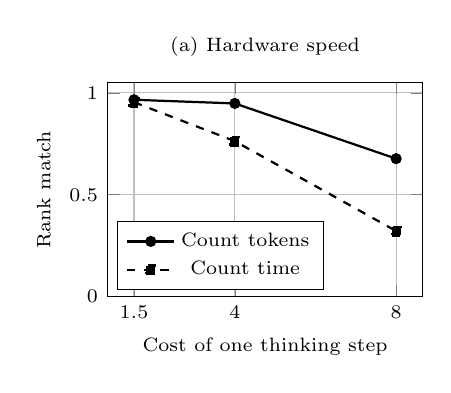
\begin{tikzpicture}
\begin{axis}[width=0.46\textwidth,height=4.3cm,title={\scriptsize (a) Hardware speed},xlabel={Cost of one thinking step},ylabel={Rank match},
 ymin=0,ymax=1.05,xtick={1.5,4,8},grid=major,legend pos=south west,
 legend style={font=\scriptsize},tick label style={font=\scriptsize},label style={font=\scriptsize},
 every axis plot/.append style={thick,mark size=1.6pt}]
\addplot[black,mark=*] coordinates {\CoordsHwTok};
\addplot[black,mark=square*,dashed] coordinates {\CoordsHwTime};
\legend{Count tokens,Count time}
\end{axis}
\end{tikzpicture}\hfill
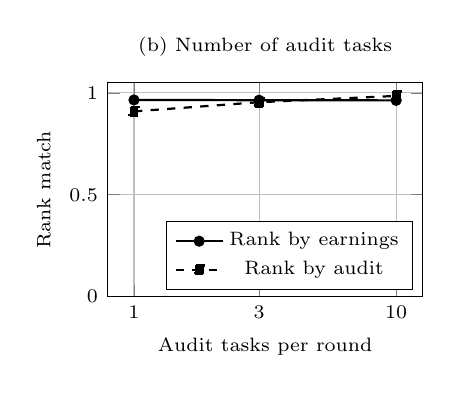
\begin{tikzpicture}
\begin{axis}[width=0.46\textwidth,height=4.3cm,title={\scriptsize (b) Number of audit tasks},xlabel={Audit tasks per round},ylabel={Rank match},
 ymin=0,ymax=1.05,xmode=log,xtick={1,3,10},xticklabels={1,3,10},grid=major,legend pos=south east,
 legend style={font=\scriptsize},tick label style={font=\scriptsize},label style={font=\scriptsize},
 every axis plot/.append style={thick,mark size=1.6pt}]
\addplot[black,mark=*] coordinates {\CoordsProbeOne};
\addplot[black,mark=square*,dashed] coordinates {\CoordsProbeTwo};
\legend{Rank by earnings,Rank by audit}
\end{axis}
\end{tikzpicture}
\caption{Rank match under the shared-tax rules (strong colony). (a) Ten computers with different speeds: counting time breaks the ranking once thinking costs more. (b) The audit score needs enough tasks: with one task per round, ranking by earnings does better.}
\label{fig:results}
\end{figure*}

\subsection{Other checks}
\textbf{Thinking depth.} Players that choose how deeply to think do better when words cost more. At the highest price, players with fixed depth run out of points after about \NDepthFixedEight{} rounds, while adaptive players last about \NDepthAdaptiveEight{} of 60.

\textbf{Parameter sweeps.} We changed the tax, the sharing rate, the removal period, the number of audit tasks, the number of paid tasks, the reward, the colony size, and the spread of skills. The audit-based rule M2 beat M0 in all \NSweepCount{} cases we ran (\NSweepBelow{} exceptions; median gain \NSweepMedian{}, smallest \NSweepMin{}). M0 fails when income is low (reward 10 gives \NLowIncomeMzero{}). With only one audit task per round, ranking by earnings does better (\NProbesOneOne{} against \NProbesOneTwo{}).

\textbf{Smarter players.} A player that plans six rounds ahead holds back even more under M0 (effort \NMidEffLook{}). The audit rule M2 stays at about the same level.

\section{The Open Tool and First Tests}
\label{sec:engine}
\textbf{The tool.} Our open engine gives agents auto-graded tasks of four kinds: arithmetic chains, modular powers, digit sums, and Collatz steps. It counts all text an agent writes, including hidden thinking, with one fixed letters-per-word rule. This treats models with different tokenisers the same. Every event goes into a log with a running hash, so a run with the same seed repeats exactly. The code has 25 tests, and it agrees with the simulator.

\textbf{First tests.} We ran three short colonies of two copies of one 8B reasoning model plus two scripted agents (Table~\ref{tab:live}). These runs check the tool. They tell us nothing about model behaviour.

\begin{table}[!t]
\caption{First tests with a local model (language-model agents only). ``Plan share'' is the share of spending on planning. ``Plan cut off'' counts planning answers stopped by the length limit.}
\label{tab:live}
\centering
\small
\begin{tabular}{@{}rrccccc@{}}
\toprule
Run & Rounds & Right & Cut off & Plan share & Plan cut off & Letters/token \\
\midrule
1 & 6 & 19/19 & 0 & n/a & n/a & 2.70 \\
2 & 4 & 8/15 & 7 & 43\% & 0/8 & 1.99 \\
3 & 3 & 11/12 & 1 & 23\% & 6/6 & 1.93 \\

\bottomrule
\end{tabular}
\end{table}

\textbf{What we learned.}
(1) The tool must count hidden thinking, which the server returned in a separate field.
(2) Run 1 tasks were too easy (19 of 19 right). Harder tasks gave 8 of 15 in run 2.
(3) A length limit cut off 7 of 15 answers in run 2, so those misses show the limit, not skill. Cut-offs must be reported on their own.
(4) Planning took 43\% of spending in run 2, and in run 3 every planning answer was cut off, so each plan was a default. Defaults must be logged.
(5) Letters per token ranged from 1.9 to 2.7, so counting letters is a fair way to price text, but it does not map to real tokens with one constant.

\section{Plan for the Real Study}
We will draw colonies of ten agents at random from several open models. The arms are the original rule M0, the audit rule M2, and a bare tournament. We will test three ideas. (H1) Under M0, agents in ranks 4--5 bunch just below rank 3, but not under M2. (H2) The rank match against an independent skill test is higher under M2 than under M0, and the bare tournament shows how much comes from the economy itself. (H3) When thinking costs more, agents think less, and ranking by earnings hurts efficient agents. We will run at least 20 colonies per arm, report cut-offs and defaults separately, combine results with a Plackett--Luce model \cite{murphy2026agentisland}, and never let a model judge its own family.

\section{Limits}
We have no results from a full study with real models. The simulated players are scripts, and the numbers were chosen to look like the reference setup, so only the directions are safe to trust. The audit score works like a plain test inside the economy, and a bare tournament matches it, so the economy must still show it adds something (H3). We tried only arithmetic-style tasks. Trading, teaming up, and cheating on the audit are not tested yet.

\section{Conclusion}
The rules of a survival game decide what its ranking means. A rank tax pays players to hold back. Counting time lets slow computers lose. Removing weak players slowly fixes most of the problem, and a bare tournament does the same. The open tool and the plan make the real test possible: does the economy show anything that a plain test does not?

\section*{Acknowledgment and AI Use}
The tool, the simulator, the scripts, and this draft were made with a lot of help from an AI system (Claude, Anthropic). The authors must check every number and proof. \todo{authors: confirm wording and funding}

\bibliographystyle{IEEEtran}
\bibliography{references}

\end{document}
